
\begin{frame}
\frametitle{Axis encoding: motivación}
\begin{figure}[h]
\centering
\subfloat[\centering $\white$ White]{{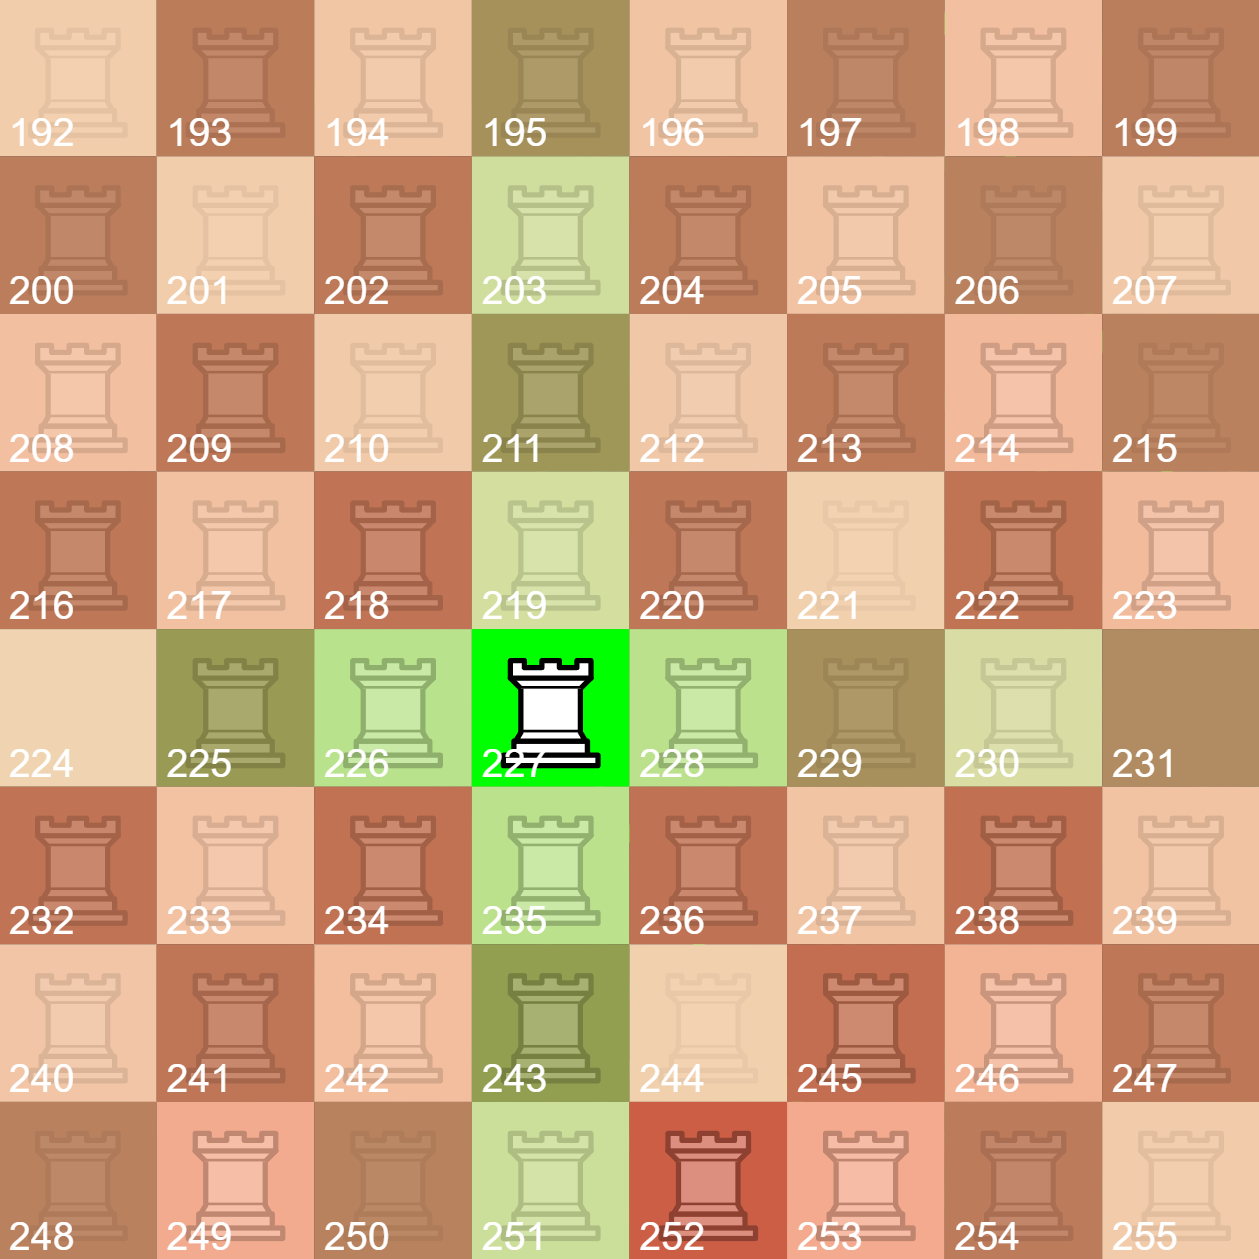
\includegraphics[width=4.4cm]{../assets/results/piece_weights/white_rook_weights.png} }}%
\qquad
\subfloat[\centering $\black$ Black]{{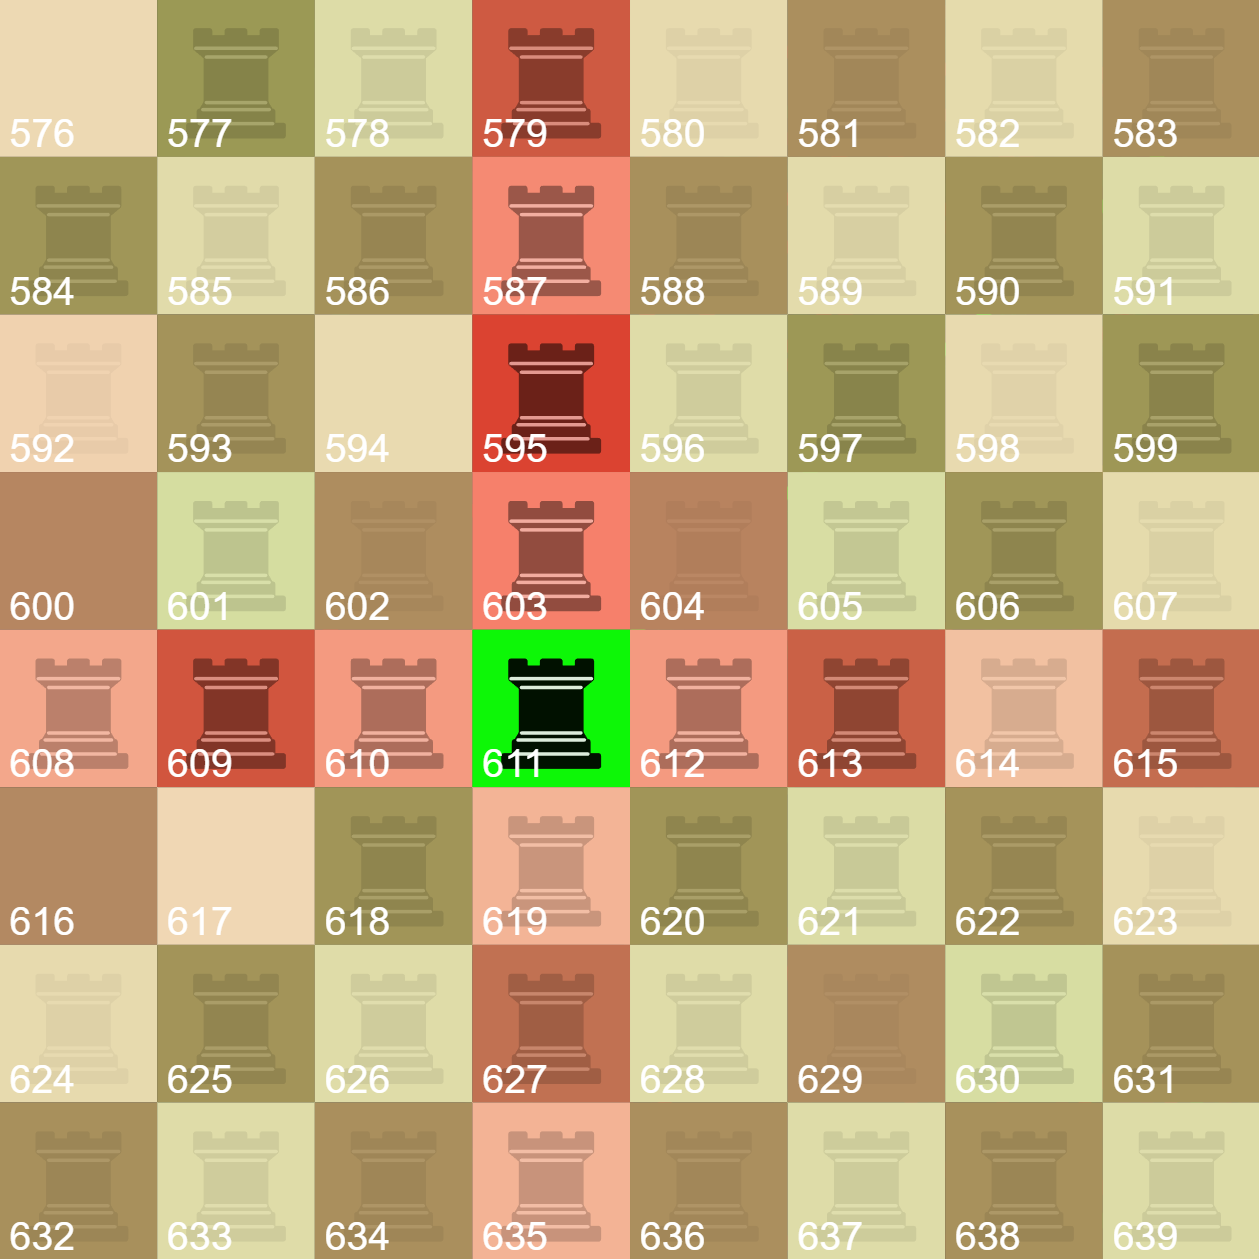
\includegraphics[width=4.4cm]{../assets/results/piece_weights/black_rook_weights.png} }}%
\caption{Weights of \textbf{a neuron} in the L1 layer, which are connected to features in \featureset{All} where the role is $\rook$ Rook. The intensity represents the weight value, and the color represents the sign (although not relevant).}
\label{fig:rook_weights}
\end{figure}
\end{frame}

\begin{frame}
\frametitle{Axis encoding: motivación}
La red detecta patrones parecidos a los movimientos de las piezas. \pause \\

Para hacerle la vida más fácil a la red, propongo agregar features como:

\begin{center}
\enquote{\textit{there is a $\white$ White $\rook$ Rook in the 4th rank}}
\end{center}

\end{frame}


\begin{frame}[shrink=5]
\frametitle{Axis encoding: experimento}
\begin{table}
\centering
\begin{tabular}{cccc}
\depiction{H} & \depiction{V} & \depiction{D1} & \depiction{D2} \\
Horizontal & Vertical & Diagonal 1 & Diagonal 2 \\
(across files) & (across ranks) &  & 
\end{tabular}
\end{table}
\pause
\begin{table}
\small
\centering
\newcommand{\fullrolecolor}{$\times$ $\featureset{Roles} \times \featureset{Colors}$}
\begin{tabular}{cccccc}
\toprule
\bf Depiction & \bf Block name & \multicolumn{2}{c}{\makecell{\bf Definition}} & \bf \makecell{Number of\\features} \\
\toprule
\depiction{H} & $\featureset{H}$ & $(\featureset{Files}$ & \fullrolecolor$)_{P}$ & 96 \\
\depiction{V} & $\featureset{V}$ & $(\featureset{Ranks}$ & \fullrolecolor$)_{P}$ & 96 \\
\depiction{D1} & $\featureset{D1}$ & $(\featureset{Diags1}$ & \fullrolecolor$)_{P}$ & 180 \\
\depiction{D2} & $\featureset{D2}$ & $(\featureset{Diags2}$ & \fullrolecolor$)_{P}$ & 180 \\
\bottomrule
\multicolumn{5}{c}{\makecell{
\vspace{-0.3cm}\\
P($\langle x, r, c \rangle$): there is a piece in $x$ with role $r$ and color $c$
}}
\end{tabular}
\end{table}
\end{frame}

\begin{frame}
\frametitle{Axis encoding: experimento}
\begin{table}[h]
\small
\centering
\begin{adjustbox}{max width=\textwidth}
\newcommand{\rolecolor}{$\times$ $\featureset{R}_{P} \times \featureset{C}_{P}$}
\begin{tabular}{ccc}
\toprule
\bf Depiction & \bf Feature set & \bf \makecell{Number of\\features} \\
\toprule
\depiction{H} $\oplus$ \depiction{V} & $\featureset{H} \oplus \featureset{V}$ & 192 \\
\midrule
\depiction{D1} $\oplus$ \depiction{D2} & $\featureset{D1} \oplus \featureset{D2}$ & 360 \\
\midrule
\depiction{H} $\oplus$ \depiction{V} $\oplus$ \depiction{D1} $\oplus$ \depiction{D2} & $\featureset{H} \oplus \featureset{V}$ $\oplus$ $\featureset{D1} \oplus \featureset{D2}$ & 552 \\
\midrule
% ------------------------------------
\midrule
\featureset{All} $\oplus$ \depiction{H} $\oplus$ \depiction{V} & $\featureset{All} \oplus \featureset{H} \oplus \featureset{V}$ & 960 \\
\midrule
\featureset{All} $\oplus$ \depiction{D1} $\oplus$ \depiction{D2} & $\featureset{All} \oplus \featureset{D1} \oplus \featureset{D2}$ & 1128 \\
\midrule
\featureset{All} $\oplus$ \depiction{H} $\oplus$ \depiction{V} $\oplus$ \depiction{D1} $\oplus$ \depiction{D2} & \featureset{All} $\oplus$ \featureset{H} $\oplus$ \featureset{V} $\oplus$ \featureset{D1} $\oplus$ \featureset{D2} & 1320 \\
\bottomrule
\end{tabular}
\end{adjustbox}
\end{table}
\end{frame}


\begin{frame}[shrink=2]
\frametitle{Axis encoding: resultados}
\begin{table}[h]
\centering
\begin{adjustbox}{max width=\textwidth}
\begin{tabular}{cccccc}
\toprule
\bf Feature set  & \bf \makecell{Number\\of features} & \makecell{\bf Val. loss\\\textit{min}} & \makecell{\bf Rating\\\textit{elo (rel. to \featureset{All})}} & \makecell{\bf Puzzles\\\textit{move acc.}} \\
\toprule
\depiction{H} $\oplus$ \depiction{V} & 192 & 0.005810 & -384.3 $\pm$ 5.1 & 0.8618 \\
\midrule
\depiction{D1} $\oplus$ \depiction{D2} & 360 & 0.006707 & -444.1 $\pm$ 5.1 & 0.8517 \\
\midrule
\makecell{\depiction{H} $\oplus$ \depiction{V} $\oplus$ \\ \depiction{D1} $\oplus$ \depiction{D2}} & 552 & 0.003907 & -183.5 $\pm$ 4.1 & 0.8748 \\
\midrule
% ------------------------------------
\midrule
\featureset{All} (reference) & 768 & 0.003134 & \textbf{0.0} & 0.8865 \\
\midrule
\featureset{All} $\oplus$ \depiction{H} $\oplus$ \depiction{V} & 960 & 0.003082 & -27.1 $\pm$ 4.1 & 0.8851 \\
\midrule
\featureset{All} $\oplus$ \depiction{D1} $\oplus$ \depiction{D2} & 1128 & 0.003087 & -26.1 $\pm$ 3.8 & 0.8814 \\
\midrule
\makecell{\featureset{All} $\oplus$ \depiction{H} $\oplus$ \depiction{V} \\ \hspace{0.75cm} $\oplus$ \depiction{D1} $\oplus$ \depiction{D2}} & 1320 & \textbf{0.003067} & -58.7 $\pm$ 3.7 & 0.8766 \\
\bottomrule
\end{tabular}
\end{adjustbox}
\end{table}
\end{frame}
